\begin{sagesilent}
import matplotlib.pyplot as plt
import numpy as np

d = np.recfromcsv("dati/", verbose=False)
d.sort()

plt.clf()
plt.ylim(ymin=3, ymax=15)
plt.title("Grafico 1")
plt.xlabel("Frequenza (Hz)")
plt.ylabel("Corrente (mA)")
plt.grid(True, which='both')
plt.loglog(d['frequenza_hz'], d['i_ma'], '.r')
plt.savefig("grafici/C2-1.png")

plt.clf()
plt.ylim(ymin=0.3, ymax=1.5)
plt.grid(True, which='both')
plt.title("Impedenze")
plt.loglog(d['frequenza_hz'], d['valore_mu']/d['v_rms'], '.r')
plt.savefig("grafici/C2-2.png")
\end{sagesilent}


\chapter{Microonde}

\section{Riflessione}

Obiettivo: verificare la legge di Cartesio utillizando la lastra di mettallo, posizionata su un supporto magnetico sul
goniometro, come superficie riflettente

\begin{center}
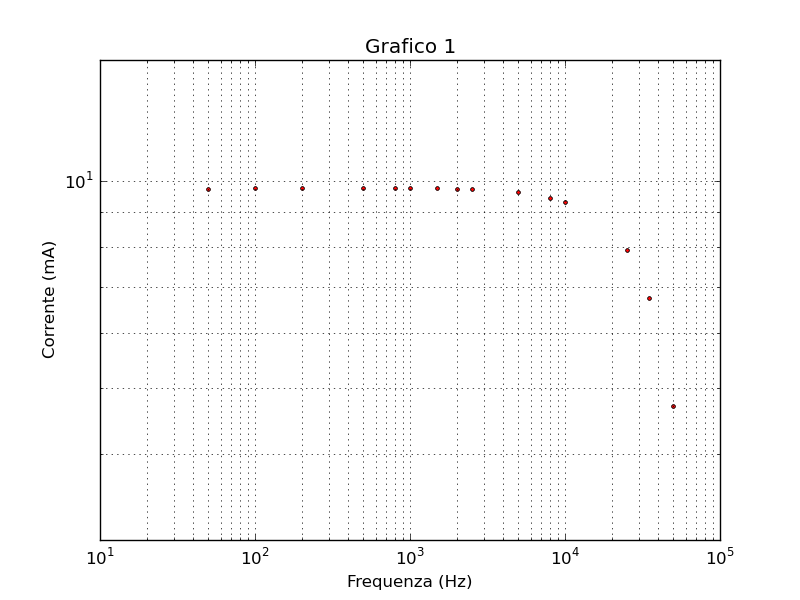
\includegraphics[scale=0.75]{grafici/C2-1.png} 
\end{center}

\section{Misura della lunghezza d'onda}
Obiettivo: posizionando emettitore e ricevitore ai capo del metro e muovendo il ricevitore lungo questo si osserva il
passaggio alterno per massimi e minimi di intensità, partendo da un massimo di intensità e spostandosi di n minimi fino ad
un altro massimo si può usare la formula
$$d = n\frac{\lambda}{2}$$
per ricavare la lunghezza d’onda.


\begin{center}
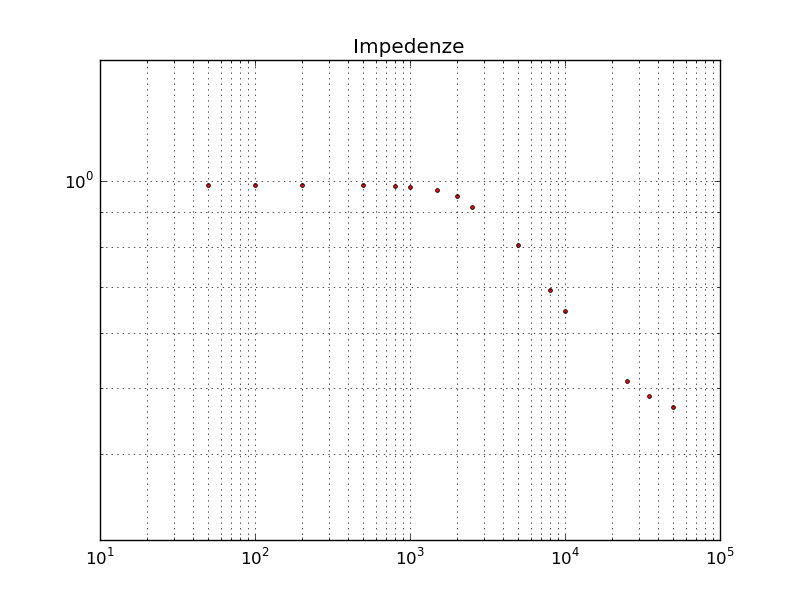
\includegraphics[scale=0.75]{grafici/C2-2.png} 
\end{center}

\section{Rifrazione attraverso un prisma}

\section{Interferenza da doppia fenditura}
Preparazione: utilizzando un supporto magnetico sul goniometro, montare tra lastre di metallo in modo da avere due
fenditure di circa 1,5 cm. Spostando il ricevitore si troveranno i massimi e i minimi di interferenza e si potrà verificare la
loro posizione rispetto alla previsione teorica: $d \sin(\theta) = n λ$ (per i massimi, con d distanza delle fenditure, $\theta$ angolo
rispetto alla perpendicolare, n numero intero).

\section{Specchio di Lloyd}
L'obiettivo del nostro esperimento è misurare la velocità della luce $c$.

L'apparato di misurazione consiste principalmente in:

\section{Analisi dati}

\section{Allegato: dati}
\begin{sagesilent}
def stampa_dati(wa, header):
  s = r"\begin{tabular}{c*{" + "%d" % (len(wa.dtype)-1)
  s += r"}{|c}}"
  s += "%s \\\\" % (header)
  s += r"\midrule"
  for i in range(0, len(wa)):
    a = ["%s" %x for x in d[i]]
    s += "%s \\\\" % join(a, "&")
  s += r"\end{tabular}"
  return s
\end{sagesilent}

\begin{center}

\sagestr{stampa_dati(d, r"Frequenza (Hz) & I (mA) & Valore mu & $V_{rms}$ (V)")}
\end{center}

